\chapterA{Investigación}

\section{Introducción}

Para poder diseñar una aplicación correctamente, es muy importante realizar previamente una investigación para saber qué
es lo que realmente se necesita, y cuáles son los problemas de nuestro público objetivo. Hay muchas maneras de conseguir esto, pero en nuestro
caso, como desgraciadamente no disponemos del tiempo para poder usar todos los métodos, hemos realizado las siguientes.

\begin{itemize}
    \item \textbf{Entrevistas.} Es una de las partes más importantes de la investigación. Con estas entrevistas podremos sacar distintos tipos de usuarios y distintos casos de uso de los mismos. Aspiramos a tener 6 entrevistas.
    \item \textbf{Cuestionarios.} Con estos cuestionarios podemos conseguir una información más cerrada. Esta información puede ser interesante para comparar nuestra idea contra otras aplicaciones existentes en el mercado.
\end{itemize}



Pero antes de realizar esta labor, debemos saber reconocer cuál es el público objetivo de nuestra aplicación y
de qué manera podemos clasificar a los distintos perfiles dentro de los clientes potenciales. Para eso hemos realizado la
\textbf{Hipótesis de personas}.

\section{Hipótesis de personas}

En esta primera fase de investigación, el primer paso que vamos a seguir es la identificación de los posibles usuarios que vamos a tener
en nuestra aplicación. Nuestro principal objetivo, como hemos visto anteriormente, es ofrecer una herramienta que permita a las personas con
discapacidad intelectual tener la posibilidad de utilizar un comparador de viajes sin problemas. Los principales usuarios que hemos identificado
y los cuáles vamos a entrevistar en la posterior fase de entrevistas son los siguientes:

\begin{itemize}
    \item\textbf{Gente que viaja por negocio.} Gente que tiene que planear viajes por motivos laborales, bien sea para viajes nacionales o internacionales. Normalmente serán viajes individuales.
    \item\textbf{Gente que viaja por ocio.} Personas que viajan por turismo, normalmente en grupo.
    \item\textbf{Gente que viaja para ver a sus familiares.} Viajero recurrente.
\end{itemize}

Por otro lado, vamos a tener otros tipos de personas identificados, que no van a ser usuarios potenciales de nuestra aplicación pese a pertenecer a 
alguno de los anteriores grupos, por lo que en el momento que detectemos que se trata de una persona encuadrada en uno de estos tipos
vamos a finalizar la entrevista ó el cuestionario, ya que no vamos a poder extraer información de valor para nuestra aplicación.


\begin{itemize}
    \item {\textbf{Usuarios que prefieren viajar con todo planificado por una agencia.}} Se trata de aquellos usuarios que cada vez que quieren
        reservar un viaje no les importa realizar un gasto extra y prefieren que todo sea organizado por una agencia de viajes, sobre todo de cara a
        evitar la aparición de ciertos conflictos que pueden tener con otras aplicaciones de la competencia.
    \item {\textbf{Usuarios que no les guste viajar y no tengan la necesidad.}} Existen usuarios que no les gusta viajar y que además nunca se han visto
        (ni se van a ver en un futuro próximo), por lo que no nos van a resultar de interés para la aplicación, ya que el objetivo buscado son perfiles que
        hayan experimentado el proceso y puedan contarnos aquellos inconvenientes que han podido encontrarse a lo largo del proceso.
\end{itemize}
 
A modo de conclusión, los perfiles de usuario que tenemos, como se puede apreciar está influenciado por dos factores muy importantes: la necesidad (o ausencia de ella) para viajar; gente que viaja por motivos laborales o familiares y gente que viaja por placer y ocio, y

\section{Plan de investigación}

Para la investigación de \textit{\app} usaremos dos técnicas: entrevistas y cuestionarios. En las subsecciones \ref{subsec:entrevistas} y \ref{subsec:cuestionarios} hablaremos en detalle del número de instancias de cada técnica y de sus distintos objetivos en más detalle.

\subsection{Entrevistas} \label{subsec:entrevistas}

Las entrevistas serán el método principal de obtención de datos. Con las entrevistas podremos ver usuarios potenciales (y no potenciales) para la aplicación y podremos hacer preguntas con mayor detalle. Se fija el objetivo en 4 entrevistas.

Las tareas a realizar en las entrevistas son:
\begin{itemize}
    \item Crear un guion de entrevista con diversas preguntas para los distintos tipos de usuarios. Esta tarea se hizo el primer día tras conocer el proyecto y se encargaron en su mayoría Pablo y Javier, aunque todo el grupo estuvo implicado. Se le dedicó solo ese día.
    \item Reclutar usuarios de distintos clases para poder tener una imagen de cada tipo de usuario de la aplicación. De esta tarea se encargaron Sergio y Leire y se ha hecho durante todo el proyecto.
    \item Entrevistar a los usuarios. Esta tarea la han llevado a cabo Daniel, Javier y Sergio en su mayoría. Se ha hecho durante todo el proyecto y se le ha dedicado aproximadamente 5 horas.
    \item Resumir las entrevistas y sacar los datos más importantes de las mismas. Pablo y Laura han sido los encargados de este apartado, se han hecho justo después de cada entrevista. Se le ha dedicado otras 7 horas a este apartado.
    \item Realizar el mapa de empatía de cada usuario entrevistado. Guillermo se ha ocupado de los mapas de empatía de todas las entrevistas. Se le ha dedicado a esta tarea 4 horas.
\end{itemize}

\subsection{Cuestionarios} \label{subsec:cuestionarios}

Los cuestionarios son nuestro método de sacar una información más guiada, para corroborar hipótesis sobre el diseño que teníamos o para ver que se nos ha podido escapar. Hemos escogido unos 30 usuarios como meta.

Las tareas a realizar en los cuestionarios son:
\begin{itemize}
    \item Crear el cuestionario y dividirlo en secciones. Leire, Rodrigo y Alejandro se han encargado en su mayoría de la creación del cuestionario. Se le dedicó 3 horas a esta tarea y se realizó el día 2 de octubre.
    \item Distribuir el cuestionario por distintos medios para alcanzar una gran cantidad de usuarios. Tanto Alejandro como María se dedicaron a difundir estos cuestionarios por distintos grupos y correos. Se le dedicó media hora a esta tarea.
    \item Analizar los datos y sacar conclusiones. Alejandro se dedicó al análisis de datos de este cuestionario. Se dedicó una hora a esta tarea.
\end{itemize}

\subsection{Distribución de tareas}

Aunque hemos sido flexibles con la asignación de tareas, pondremos aquí un resumen de las tareas que ha hecho cada uno a parte de las mencionadas en el apartado anterior:

\begin{itemize}
    \item Análisis de la competencia. Daniel y Carlos se dedicaron a esta tarea. La tarea se realizó en en torno a 2 horas.
    \item Listado de factoides. María, Leire, Laura  y Rodrigo hicieron los distintos listados. Se dedicó un total de 4 horas en conjunto para hacerlo.
\end{itemize}

%%%%%%%%%%%%%%%%%%%%%%%%%%%%%%%%%%%%%%%%%%%%%%%%%%%%%%%%%%%%%%
\section{Entrevistas}
%%%%%%%%%%%%%%%%%%%%%%%%%%%%%%%%%%%%%%%%%%%%%%%%%%%%%%%%%%%%%%

Es la parte más importante de la investigación, ya que es de donde conseguiremos obtener más información. Consiste en realizar una serie de preguntas al usuario para
ver si encaja con los perfiles objetivo de nuestra aplicación, y en caso de hacerlo, obtener los datos necesarios para poder diseñarla. Gracias a esto podremos averiguar
cuáles son los problemas que tienen estas personas con los comparadores actuales y qué necesidades tendrían.

Tenemos distintos clientes que forman parte de nuestra hipótesis de personas, y ambos tienen necesidades distintas. Por tanto tendremos distintas preguntas
dependiendo del perfil al que nos enfrentemos.

Todas las entrevistas comenzarán presentándonos y preguntando el nombre al entrevistado. Tras eso, tendremos que pedir autorización para grabar imágenes, ya que las
grabaciones son necesarias para un posterior análisis y recabar así la mayor cantidad de información posible. Para que la entrevista sea más distendida, preguntaremos
si le podemos tutear. Tras esto, explicaremos nuestros objetivos con la aplicación y procederemos a realizar las preguntas.

\subsection{Preguntas a usuarios}

Al comienzo realizaremos el denominado como \textit{Screener}, es decir, una serie de preguntas para ver si el entrevistado es un cliente potencial. En caso de serlo,
podremos proceder con el resto de preguntas.

\begin{enumerate}
    \item {\textbf{?`Cuántos años tienes?}} sirve para encuadrar al usuario dentro de un marco de edad concreto y poder tratar con él en función de esto.
    \item {\textbf{?`Cómo de cómodo te sientes con la tecnología?}}
    \item {\textbf{?`Te gusta viajar? ?`Cuéntame por qué?}} es la pregunta que nos va a determinar si el usuario es potencial de la aplicación
                o si bien lo tenemos que descartar.
    \begin{enumerate}
        \item {\textit{Sí,}} usuario potencial. Tenemos que conocer ahora si le gusta viajar por ocio o bien lo tiene que hacer por negocios.
        \item {\textit{No,}} puede seguir estando dentro de la hipótesis de usuarios. En este caso las preguntas a hacer van a variar y van a
                        depender de la respuesta que nos de.
    \end{enumerate}
    \item {\textbf{?`Suele viajar?}} sirve para identificar si el usuario es apto, porque si no viaja no tiene sentido la aplicación.
    \item {\textbf{?`Le gustaría viajar más?}} sirve para saber si el usuario que no viaja tiene pensado viajar en un futuro y por tanto, considerarlo apto.
    \item {\textbf{?`Disfruta cuando viaja?}} sirve para entender al usuario que viaja y si va a usar la aplicación más o menos frecuente.
    \item {\textbf{?`Cuál es tu medio de transporte favorito y por qué?}} sirve para entender al usuario que viaja y si va a usar la aplicación más o menos frecuente.
    \item {\textbf{?`Qué tipo de viajes has hecho?}} sirve para entender al usuario que viaja y si va a usar la aplicación más o menos frecuente.
    \item {\textbf{?`Sueles viajar acompañado?}} tenemos que tener en cuenta si la persona con la que estamos tratando requiere de la
                ayuda de un acompañante que viaje con él para tenerlo en cuenta a la hora de desarrollar la aplicación y nos ayuda a conocer un poco al entrevistado.
    \item {\textbf{?`Por qué motivos suele viajar?}} sirve para identificar las motivaciones del usuario.
    \item {\textbf{?`Qué es lo que más le dificulta a la hora de viajar? ?`Hay algo más que le dificulte viajar?}} sirve para identificar molestias que tiene
                el usuario al planificar un viaje.
    \item {\textbf{?`Cuando vas a organizar un viaje, que es lo primero que haces?}}
    \item {\textbf{?`Te encargas tú de organizar el viaje?}} queremos conocer si el usuario tiene la iniciativa para organizar el viaje por sí solo o bien si
                recurre a profesionales como agencias de viajes o a terceras personas.
    \item{ \textbf{?`Cómo has organizado tus viajes?}}
    \begin{enumerate}
        \item {\textit{No:}} ?`No has pensado nunca en usar un comparador de viajes? queremos conocer si aunque el usuario recurra a agencias de viajes o
                        a otras personas para realizar el viaje usaría en algún momento nuestra aplicación.
        \item {\textit{Si:}} ?`Te has encontrado alguna dificultad en el proceso? está bien para finalizar el screener e introducir la siguiente parte.
    \end{enumerate}
    \item {\textbf{?`Te resulta más cómodo realizar estas búsquedas de viajes en una aplicación móvil o en una página web?}}
    \item {\textbf{?`Cuál es el factor clave que hace que se decante por esa opción en un viaje?}} sirve para saber sus prioridades.
    \item {\textbf{?`Influye el coste del viaje en su elección?}} sirve para saber más información.
    \item {\textbf{?`Cuál de las partes de una página tradicional de comparación de viajes te parece más tediosa?}} necesitamos conocer los problemas que
                puede encontrarse el usuario en las páginas tradicionales para tenerlo en cuenta y poder mejorarlo en nuestra aplicación. En caso de que
                la respuesta sea afirmativa, podemos preguntarle si existe alguna opción de ayuda dentro de la plataforma.
    \item {\textbf{En caso de que hayas tenido algún problema en estas páginas, ?`has podido solicitar ayuda de manera sencilla?}}
    \item {\textbf{?`Según tu opinión, ?`cómo debería ser la forma ideal en la que una aplicación muestre la información?}}
    \item {\textbf{?`Hay alguna función de las páginas tradicionales que consideres útil para tus necesidades?}}
    \item {\textbf{En caso de que hayas realizado alguna reserva de viaje, ?`has conocido y sido informado de forma clara de las condiciones
                        y políticas de cancelación del viaje?}}
    \item {\textbf{?`Te gustaría que estas páginas incluyesen más información sobre accesibilidad para viajeros con discapacidad?}}
    \item {\textbf{?`Podrías darme algún ejemplo de aplicación que te guste y uses a diario?}}: queremos poner al usuario en una situación
    en la que nos comente una aplicación que le guste para poder conocer los motivos que le llevan a ello.
    \item {\textbf{?`Consideras que es una aplicación accesible??`Por qué?}}: queremos conocer desde el punto de vista de la persona aquellos
    elementos y problemas que puede identificar dentro de la aplicación y que puedan suponer un problema.
    \item {\textbf{Acordarse de hacer el debriefing, para hacer un repaso de lo que ha dicho a ver si se acuerda de algo más.}}
    \item {\textbf{?`Se te ocurre algo más de lo que hemos hablado que podría ayudarnos?}}
\end{enumerate}

Al finalizar, le agradeceremos al entrevistado su tiempo y su participación en nuestro proyecto.


\subsection{Resúmenes de entrevistas}

\textbf{Entrevista 1 - Madi:} Entrevista hecha por videollamada\footnote{Enlace a la entrevista 1: \url{https://drive.google.com/file/d/1a6UrtghooaZqYAVYK9umbhKor8_vxPM1/view?usp=drive_link}}. Participantes: Daniel, Sergio, Leire y Guilermo, duración 19:21.

Resumen de entrevista, el mapa de empatía está representado en la figura \ref{fig:mapa_madi}.

\begin{itemize}
    \item FEDDI, está como secretaria pero se encarga de gestionar los viajes (horarios y logística) para llevar a los competidores.
    \item Lleva 16 años trabajando con ellos.
    \item Trabajo de campo: Prepara la mesa de premiación y eventos deportivos.
    \item Trabajo administrativo: Licencia, gestión de cara al público, pagar tasas…
    \item Las autonomías se gestionan del desplazamiento.
    \item Alrededor de 4 competiciones de natación y 5 de atletismo.
    \item Las personas con DI se manejan mal con el tema de aplicaciones, internet o necesitan acompañante.
    \item Pueden necesitar acompañante sobre todo por problemas de orientación.
    \item Busca en las páginas de las compañías que pueden salir baratos o con Renfe.
    \item Trabaja con una agencia (betravel).
    \item No usa un comparador porque ya tiene localizadas las compañías que funcionan correctamente con los destinos que frecuenta.
    \item Ryanair por ejemplo no lo usa porque puede retrasarse y te cobran por la maleta.
    \item Se fija en el precio, en los horarios y se asegura de que puedan ir los acompañantes.
    \item Aerolíneas:
    \begin{itemize}
        \item Nacional: AirEuropa, Iberia.
        \item Tren: Renfe.
    \end{itemize}
    \item Que la aplicación sea lo más simple posible para la gente con DI.
    \item Que sea más simple mirar los servicios que ofrece la compañía.
    \item Que exista una alerta para saber cuándo tienen que bajar del tren y así no se pierdan (esa es buena).
    \item Normalmente el servicio de acompañante tiene coste adicional. AENA lo da de forma gratuita, pero mucha gente no lo sabe y la gente paga el precio extra de la compañía (también está bien).
\end{itemize}


Transcripción resumen con marcas de tiempo:

\noindent\textbf{0:00 -- 0:08 $\rightarrow$} Presentación, se llama Madi y es la secretaria de la fundación. \\
\textbf{0:10 -- 0:18 $\rightarrow$} Madi da su consentimiento para grabar la entrevista. \\
\textbf{0:20 -- 1:00 $\rightarrow$} Daniel presenta el proyecto a Madi y nos cuenta que ella es la persona que se encarga de organizar los viajes para deportistas de alta competición. \\
\textbf{1:05 -- 2:00 $\rightarrow$} Daniel pregunta “Nos podrías comentar que es lo que haces tu en esta asociación y que es la asociación en concreto” Madi responde que la asociación FEDDI es la federación española de deportes para personas con discapacidad intelectual, ella como secretaria se encarga de si hay alguna concentración deportiva o algún evento internacional ella dice que no es como una agencia de viajes sino que se encarga de cuadrar horarios para tema logística de la organización y sacar los billetes a través de renfe o de alguna aerolínea o de derivar a una agencia de viajes. \\
\textbf{2:02 -- 2:14 $\rightarrow$} Daniel pregunta cuánto tiempo lleva trabajando en FEDDI, lleva 16 años trabajando con ellos. \\
\textbf{2:15 -- 4:36 $\rightarrow$} Daniel pregunta cómo es trabajar en esta federación y trabajar con personas con esta discapacidad en el dia a dia, Madi comenta que hay dos campos, el trabajo de campo y el trabajo administrativo, ella va a los 3 campeonatos más importantes, que tienen más participantes, en la práctica, ella lleva tema protocolo, entrega de medallas y pasando resultados deportivos, ella disfruta más el trabajo de campo por el trato con los deportistas. Comenta que en el trabajo administrativo lleva facturación, certificados, licencias y trabajo de cara al público. Ella se siente gratificada con el trabajo en el campo. \\
\textbf{4:40 -- 6:39 $\rightarrow$} Daniel le pregunta cómo es en el trabajo de campo, son los viajes y como es llevarlos a cabo con las personas con discapacidad, Madi comenta que en los campeonatos de españa, los clubes son los encargados del desplazamiento de los deportistas, ella interviene poco o nada. Ella se encarga más de los campeonatos internacionales, ella les recepciona, les recoge y les lleva al punto de encuentro, donde se reúne toda la selección. Comenta que hay bastantes campeonatos. \\
\textbf{6:45 -- 7:43 $\rightarrow$} Daniel pregunta que qué problemas tendrán los deportistas a la hora de organizar los viajes si tuviesen que organizarlos ellos, utilizando páginas como kayak, Madi responde que sus atletas el problema principal es la dependencia, que no se manejan bien con las aplicaciones y con internet, para desplazarse algunos necesitan un acompañante \\
\textbf{7:45 -- 8:30 $\rightarrow$} Daniel pregunta qué motivos piensa que necesitan un acompañante y qué problemas se pueden encontrar durante el viaje, Madi comenta que en el aeropuerto a la hora de hacer el check in en el aeropuerto y encontrar la puerta de embarque, tienen problemas para orientarse y no todos se manejan bien. \\
\textbf{8:31 -- 9:07 $\rightarrow$} Daniel pregunta qué problemas tienen con las tecnologías, Madi comenta que los atletas son dependientes de los padres y de los entrenadores, depende mucho del grado de discapacidad. \\
\textbf{9:09 -- 10:02 $\rightarrow$} Daniel le pregunta que qué utiliza a la hora de organizar los viajes, si utiliza ella de manera independiente o buscando páginas que ya existen. Ella no usa aplicaciones, se mete en la página web de la aerolínea donde sabe que los transportes le van a salir más económicos, Air Europa, Iberia o Renfe. En caso de tener que organizar o pedir presupuesto para vuelos internacionales, utilizan una agencia de viajes que se llama betravel. \\
\textbf{10:03 -- 11:39 $\rightarrow$} Daniel pregunta por qué busca directamente en una compañía en vez de usar un comparador donde salen distintas aerolíneas. Madi responde que porque en los lugares de origen de los deportistas ya tiene localizadas dos compañías que son las que funcionan ahí, y descarta aerolíneas como ryanair por el problema de si tienes que pagar la maleta aparte, y que tiene muchos problemas de retrasos, entonces no utiliza compañías de bajo coste que no te ofrecen asistencia.  Por lo que utilizan compañías que sí ofrecen el servicio de acompañamiento de aena. Comenta que con Renfe también utilizan este sistema de acompañamiento. \\
\textbf{11:40 -- 13:02 $\rightarrow$} Daniel pregunta por más factores que tiene en cuenta a la hora de coger el billete, como por ejemplo el precio. Madi comenta que sí, el precio es uno, y miran también variedad de horarios, ya que no todas las aerolíneas tienen amplio horario, comenta que siempre sale más económico buscarlo directamente en la página que utilizar un comparador de viajes. \\
\textbf{13:03 -- 14:00 $\rightarrow$} Daniel pregunta si se fijan si se fija en que la aerolínea ofrece más facilidades a la hora de viajar, comenta que no que solo compara con lo que ya ha comentado, que como suelen ser los mismos atletas ya tiene todo bastante mecanizado. \\
\textbf{14:03 -- 14:27 $\rightarrow$} Daniel pregunta qué compañías suelen utilizar, Madi responde que a nivel nacional Air Europa, Iberia y para trenes siempre en Renfe. \\
\textbf{14:37 -- 17:37 $\rightarrow$} Daniel comienza a hacer el debriefing y pregunta si hay algo más que quiera añadir de lo que ya ha comentado para ayudarnos a diseñar la aplicación accesible para personas con discapacidad intelectual. Madi comenta que debería ser muy simple, lugar, destino y fecha. Por ejemplo, comenta que estaría bien poder ver si la compañía ofrece servicio de asistencia, ya que a los padres les da miedo que vayan solos, los que van en tren que puedan tener una alerta para que sepan cuando se tiene que bajar. \\
\textbf{17:37 -- 18:55 $\rightarrow$} Daniel comenta que ninguna aplicación que ha visto ofrece el servicio de ver si se ofrece acompañante, Madi comenta que sería importante, ya que si solicitas este servicio normalmente tiene coste, pero aena ofrece ese servicio de manera gratuita y eso no aparece en ninguna página de aerolínea y por ello es desconocido. \\
\textbf{18:57 -- 19:21 $\rightarrow$} Daniel le pregunta si se le ocurre alguna cosa más que se le ocurra para ayudarnos y no se le ocurre nada así que Daniel le da las gracias y procede a terminar la llamada.


\textbf{Entrevista 2 - Sofia:} Entrevista hecha por videollamada\footnote{Enlace a la entrevista 2: \url{https://drive.google.com/file/d/1RUf5q8dvR_aoA2IjaGYwXAqlAuBsn4sl/view?usp=drive_link}}. Participantes: Guilermo y Laura, duración 21:13.

Resumen de entrevista, el mapa de empatía está representado en la figura \ref{fig:mapa_sofia}.



Transcripción resumen con marcas de tiempo:

\noindent\textbf{00:00 -- 00:17 $\rightarrow$} Guillermo se presenta y explica brevemente el proyecto que vamos a realizar a la entrevistada, Sofía. \\
\textbf{00:18 -- 00:32 $\rightarrow$} Sofía presta su consentimiento a la grabación de la entrevista. \\
\textbf{00:33 -- 02:36 $\rightarrow$} Presentación: Sofía es estudiante, tiene 21 años y considera que tiene un buen manejo de la tecnología. Le gusta mucho viajar y considera que es uno de sus hobbies favoritos porque le gusta conocer nuevas culturas, vivir experiencias y explorar lugares desconocidos. Ha viajado por Europa, Estados Unidos y por el territorio nacional. Aunque le gustaría viajar más y está siempre en búsqueda de uno. \\
\textbf{02:37 -- 07:09 $\rightarrow$} Preguntas generales: Sofía usa diversos métodos de transporte como el coche, el transporte público, el avión y el tren, así como transporte privado, en pocas ocasiones. Normalmente suele viajar con amigos y familia por ocio. \\
\textbf{07:10 -- 07:42 $\rightarrow$} Guillermo pregunta cuáles son las dificultades que ha podido encontrar a la hora de viajar, Sofía responde que al viajar pierdes la comodidad que puedes tener en casa, pero que no ha encontrado ningún problema en particular en sus viajes más allá de la aceptación cultural. \\
\textbf{07:43 -- 08:31 $\rightarrow$} Guillermo pregunta que a la hora de reservar un viaje qué es lo primero que hace y Sofía responde mirar precios y escoger el más económico y que se adapte a sus necesidades. \\
\textbf{08:32 -- 09:17 $\rightarrow$} Guillermo pregunta si es ella quien se encarga personalmente de buscar los viajes y Sofía responde que en ocasiones sí es ella la que lo realiza, pero cuando no lo hace participa en la decisión final. \\
\textbf{09:18 -- 10:15 $\rightarrow$} Guillermo pregunta si ha usado alguna vez algún comparador de viajes y Sofía le responde que ha usado múltiples comparadores, como Kayak, SkyScanner, y busca entre las distintas páginas las mejores ofertas. \\
\textbf{10:16 -- 11:45 $\rightarrow$} Guillermo pregunta si ha encontrado alguna dificultad en alguna de las páginas mencionadas anteriormente a la hora de realizar una reserva y Sofía le contesta que por lo general no y que el único punto negativo podría ser la subida de precios después de seleccionar una opción. Como solución a este problema se propone que se indique directamente el precio final a pagar. \\
\textbf{11:46 -- 12:00 $\rightarrow$} Guillermo pregunta si le resulta más fácil utilizar estas páginas en aplicación web o en aplicación móvil y Sofía responde que suele usar el ordenador para realizar las búsquedas. \\
\textbf{12:01 -- 13:10 $\rightarrow$} Sofía realiza varias búsquedas hasta encontrar la que se adecua a sus necesidades, prefiriendo una salida a una hora temprana sabiendo que va a ahorrar dinero. \\
\textbf{13:11 -- 14:24 $\rightarrow$} Respecto a la dificultad en el proceso de comparación, Sofía se ha encontrado con algunas páginas en las que la carga es muy lenta o pinchas en un enlace y te desvía a otra página. También considera que SkyScanner es una página que está bien implementada, fácil de usar y accesible. \\
\textbf{14:25 -- 15:14 $\rightarrow$} Cuando se ha encontrado con dificultades en la búsqueda, ha desistido de usar esa aplicación y ha optado por páginas alternativas. \\
\textbf{15:15 -- 15:33 $\rightarrow$} Sofía no requiere de necesidades particulares a la hora de visualizar la interfaz, es decir, con que se use una interfaz sencilla y fácil de usar sería suficiente. \\
\textbf{15:34 -- 16:40 $\rightarrow$} Guillermo pregunta si a la hora de reservar lee las condiciones y añadidos y Sofía le responde que normalmente sí y que en muchas ocasiones son las compañías las que realizan estos añadidos y no los propios comparadores. \\
\textbf{16:41 -- 17:53 $\rightarrow$} Guillermo pregunta si considera que estas aplicaciones son accesibles para personas con discapacidad y Sofía responde que depende del grado y tipo de discapacidad. \\
\textbf{17:54 -- 18:37 $\rightarrow$} Una de las aplicaciones que Sofía usa en su día a día es Whatsapp y considera que es accesible y fácil de usar. \\
\textbf{18:38 -- 21:00 $\rightarrow$} Guillermo comienza el debriefing y le pregunta si tiene algo más que añadir. \\
\textbf{21:01 -- 21:13 $\rightarrow$} Se procede a agradecer a la entrevistada y a la finalización de la entrevista.

\textbf{Entrevista 3 - Alberto:} Entrevista hecha por videollamada\footnote{Enlace a la entrevista 3: \url{https://drive.google.com/file/d/1qqx8KDAfCw4QjHHnp4rkoky2YeaGp_I6/view?usp=drive_link}}. Participantes: Leire y Sergio, duración 17:22.

Resumen de entrevista, el mapa de empatía está representado en la figura \ref{fig:mapa_alberto}.

\begin{itemize}
    \item \textbf{Alberto}
    \item \textbf{22 años}
    \item \textbf{Sin discapacidad}
    \item Se desenvuelve bien con la tecnología (informático)
    \item Usa Whatsapp, Twitter (actualidad), YouTube, Amazon
    \item Busca chollómetro para ver ofertas
    \item Le parecen fáciles de usar.
    \item Le gusta viajar para descubrir historias, paisajes y nuevas culturas
    \item Viaja por ocio solo
    \item Viaja una vez al mes más o menos (para ir al pueblo o a Cantabria)
    \item Le gustaría viajar más (quiere salir de España)
    \item Usa vehículo propio normalmente para viajar, hace 7 años que no va en avión
    \item No usa Uber, muy ocasionalmente usa el taxi, pero prefiere el transporte público.
    \item Hace poco fue a Burgos, pero en coche
    \item Suele viajar con su pareja
    \item No tiene muchas dificultades a la hora de viajar (se prepara un itinerario de antes)
    \item Antes iba a la aventura a viajar
    \item No le resulta difícil, sobre todo le resulta tediosa
    \item Cuando viaja le gusta ir buscando el itinerario que es lo mejor para ver
    \item Hacen la organización en conjunto.
    \item Prefieren conocer la península por ahora, por eso prefieren ir en coche, su búsqueda es sobre todo de hoteles.
    \item En alojamientos se basan en:
    \begin{itemize}
        \item Que les guste visualmente
        \item Buena localización, no quieren la periferia
        \item El precio
    \end{itemize}
    \item Al usar Booking, no le gusta que Booking le obligue a escoger fechas, preferiría que le dijese el más barato sin seleccionar fechas concretas.
    \item Tiene problemas en la sobrecarga de ofertas, prefiere ver unas pocas buenas.
    \item También le gustaría que se pudiesen destacar los puntos fuertes de cada alojamiento (no solo en precio, sino también en características como "más espacioso" o "más céntrico", etc.).
    \item Si hay muchas ofertas, es muy difícil hacer que alguna destaque.
\end{itemize}


Transcripción resumen con marcas de tiempo:

\textbf{Entrevista 4 - Beatriz:} Entrevista hecha por videollamada\footnote{Enlace a la entrevista 4: \url{https://drive.google.com/file/d/1dFgLaFEXE7M9Wqg0n8dhuQINzxlIO8gy/view?usp=drive_link}}. Participantes: Sergio, Guillermo y Javier, duración 25:16.
Resumen de entrevista, el mapa de empatía está representado en la figura \ref{fig:mapa_bea}.



Transcripción resumen con marcas de tiempo:

\noindent\textbf{00:00 -- 03:00 $\rightarrow$} Beatriz es una mujer de 21 años a la que a grandes rasgos le gusta mucho viajar y que se siente muy cómoda con las nuevas tecnologías.
Ella viaja por ocio, para conocer nuevos lugares y culturas. A pesar de su gran afición por hacer turismo, Beatriz viaja poco para su gusto, todos los años viaja al pueblo de su 
familia a visitar a sus allegados. Todos los años visita otros lugares de España y es cada dos años cuando viaja a otros países. A Beatriz le gustaría viajar más y salir de España
más de una vez al año, los motivos por los que no puede hacerlo con más frecuencia es por su situación económica y el escaso tiempo que tiene de vacaciones. Cuando viaja suele 
coger coche para moverse por la península, para el resto de destinos coge el avión. Además, mayoritariamente viaja acompañada por algún familiar suyo. \\
\textbf{03:00 -- 08:00 $\rightarrow$} Lo que más le dificulta a Beatriz es reservar vuelos a precios asequibles ya que para ella prioriza el precio del vuelo ante todo. Es muy 
estresante para ella encontrar vuelos y alojamientos baratos y dentro de unas fechas concretas. Suele organizar ella sus viajes cuando va sola, cuando va con su familia, lo 
organiza todo el núcleo familiar en conjunto. Para ella no es ningún problema sacrificar algunas facilidades como el  tipo y la cantidad de equipaje que se puede llevar, el 
hecho de elegir asiento o los horarios de ida y vuelta. Para ella cuanto más barato mejor. Beatriz organizó un viaje y eligió eDreams para reservar sus vuelos. Para ella es más
cómodo coger vuelos directamente vía la página web de las aerolíneas porque lo ve más seguro, pero escogió finalmente este comparador para encontrar vuelos más baratos gracias
a una suscripción temporal gratuita. A pesar de encontrar los vuelos más baratos, fue una tarea muy tediosa la realización de la reserva. Muchos pasos y muchas pantallas 
sugiriendo añadir facilidades o ventajas a la reserva como las mencionadas antes, además estas pantallas se repetían. Otra complicación que tuvo a la hora de reservar el viaje 
es que no ponía de forma clara el aeropuerto destino de la ida u origen de la vuelta, pues eran en aeropuertos distintos. \\
\textbf{08:00 -- 15:00 $\rightarrow$} Beatriz utiliza con mucha frecuencia aplicaciones como Chrome, Whatsapp y Discord. Le preguntamos a Beatriz por qué elige Chrome antes que
cualquier otro navegador, ella responde que es un navegador que ha usado casi toda la vida y que ya tiene todo su navegador customizado y con marcadores y extensiones a su gusto, 
además es muy sencillo para ella sincronizar búsquedas e información con este buscador entre su smartphone y su ordenador. Esto nos da algunas ideas para nuestro diseño en la 
aplicación. En cuanto a comparadores, su favorito y más sencillo para ella es Google Flights, el cual conduce directamente al comparador que ofrece el vuelo más barato. Para ella
no cree que sean muy accesibles estos comparadores porque pueden estar muy cargados de información y cree que siempre intentan aprovecharse de la gente más inexperta para poder
ganar más dinero en las reservas. Hablamos con ella sobre la estética de estos comparadores y nos confirma que el que más le gusta en ese ámbito es eDreams porque está todo muy 
distinguido y más claro que en otros. Le preguntamos sobre qué le vendría mejor a ella cuando opera en estos comparadores y cree que debería poner más claro el destino y le 
gustaría también que hubiera sugerencias sobre destinos cercanos a su destino final más baratos. \\
\textbf{17:45 -- 25:16 $\rightarrow$} Por último, Beatriz considera que es importante para todo el mundo aprender a usar los comparadores de viajes o mejorar su accesibilidad 
para personas poco acostumbradas a esto. Debido al bombardeo de sugerencias y mucha “letra pequeña” muchas veces el cliente sale muy poco beneficiado en comparación a todo el 
tiempo y dinero que ha invertido en la reserva de vuelos. Beatriz resalta una incidencia que tuvo con eDreams, se trata de un problema en el que eDreams no tenía contrato para 
vender vuelos de Ryanair en su web, entonces lo que hacían era pedir toda la información personal del cliente y ellos reservaban el vuelo desde la página web de Ryanair. Por 
este motivo, Ryanair comenzó a bloquear vuelos entre ellos la reserva de Beariz, pues se estaban reservando vuelos a nombre de los clientes, por ello pidieron a los clientes 
reales una verificación tediosa que implicaba grabaciones de la cara, fotos de DNI, etc. Además esta verificación conllevaba un coste, por lo que le salió más cara la reserva 
y cree que es poco accesible para personas con pocos conocimientos y soltura con las nuevas tecnologías.
\section{Cuestionarios}

Los cuestionarios los hemos realizado finalmente con Formularios de \textit{Google}. El público objetivo de este cuestionario es gente de cualquier edad a la que le guste viajar. Este cuestionario se ha difundido por grupos de amigos, grupos de asociaciones de la facultad y a distintos familiares por \textit{Whatsapp}.

El público que buscamos para realizar este cuestionario eran personas que viajen al menos una vez al año y utilicen aplicaciones de comparación de algún tipo. Al ser un espectro bastante amplio podemos permitirnos difundir e formulario por un medio bastante amplio.

La finalidad de este cuestionario es el sacar información más concreta (frecuencia de viajes, aplicaciones usadas para estos) de un gran número de usuarios. El ``gran número'' de usuarios ha sido finalmente de 59 respuestas, de las cuales 6 son viajeros por trabajo y 52 viajantes por ocio, solo uno ha seleccionado la opción de ``otro''.

\subsection{Guión}
Las preguntas del cuestionario son las siguientes:
\begin{enumerate}
    \item\textbf{Edad.} Pregunta de screening para enmarcar el resto de la respuesta.
    \item\textbf{Género.} Una vez más, pregunta de screening.
    \item\textbf{Entorno en el que vive el encuestado.} Otra pregunta de screening para saber si el usuario vive en una ciudad o en el entorno rural.
    \item\textbf{Poder adquisitivo.} No entramos en muchos detalles, pero no es lo mismo la comparativa que puede hacer una persona con unos recursos bajos y otra con unos recursos mayores. (observación). Pregunta de screening.
    \item\textbf{Gusto por viajar.} Es importante el contexto de si te gusta o no viajar para poder entender tus frustraciones con los sistemas de comparación.
    \item\textbf{La parte buena (o la parte mala) de viajar.} Queremos conocer las partes que más frustran a los viajantes para ver si es algo que nuestra aplicación pueda solucionar.
    \item\textbf{Frecuencia de viaje.} La gente que más viaje será la que más compare (intuitivamente), así que es importante saber la frecuencia en la que viaja un encuestado para tener más perspectiva sobre su opinión.
    \item\textbf{Posibilidad de viajar más.} Queremos saber si nuestros usuarios quieren viajar más y hay algo que se lo impida.
    \item\textbf{Disfrute al viajar.} Parece similar a la  pregunta 5, pero a una persona puede no gustarle alguna parte del proceso del viaje y aun así disfrutar del resto del viaje.
    \item\textbf{Medios de transporte.} Al ser nuestra aplicación un comparador de viajes, necesitamos saber cuales son los medios de transporte más usados.
    \item\textbf{Motivos de viaje.} El viaje por ocio y el viaje por trabajo pueden presentar maneras muy distintas de como enfocar esa comparación y la forma en la que buscamos destino y medio de transporte.
    \item\textbf{Uso de herramientas y dificultad de las mismas.} Para hacer  una buena aplicación hay que conocer a la competencia, por ello queremos saber la opinión de nuestro público sobre otras aplicaciones populares.
    \item\textbf{Preguntas para gente con discapacidad:}
    \begin{enumerate}
        \item\textbf{Discapacidad, tipo (general) de discapacidad y adaptaciones.} Es importante para nosotros el saber que problemas pueden surgirle a alguien con algún tipo de discapacidad para tenerlo en cuenta en la aplicación.
    \item\textbf{Frecuencia en la que el encuestado organiza viajes.} Si el encuestado no organiza viajes es complicado que nos pueda dar mucho \textit{feedback} sobre aplicaciones de comparativa de viajes.
    \item\textbf{Dificultad en a la hora de buscar viajes y el tipo de dificultad.} No van a ser las mismas dificultades para gente con discapacidades físicas que para gente con discapacidades psíquicas.
    \item\textbf{Falta de funcionalidades en los buscadores tradicionales.} Queremos saber si los usuarios han echado en falta alguna característica en sus búsquedas.
    \end{enumerate}
    \item\textbf{Preguntas para gente sin discapacidades}
    \begin{enumerate}
        \item\textbf{Viajes en el último año.} Si un usuario ha viajado en el último año nos puede dar información bastante actualizada.
        \item\textbf{Organización del viaje.} Queremos saber si el usuario ha organizado algún viaje en el último año.
        \item\textbf{Uso de comparadores, agencias o ninguna de las dos opciones y sus principales motivos para ello.} Queremos saber si los usuarios usan comparadores y sus principales motivos para ello.
        \item\textbf{Problemas y accesibilidad de los comparadores.} Queremos saber la dificultad de los usuarios de la encuesta ante distintas características de los comparadores modernos.
        \item\textbf{Falta de funcionalidades.} Queremos saber si los usuarios han echado de menos alguna funcionalidad concreta en los comparadores tradicionales.
    \end{enumerate}
    
\end{enumerate}

Podemos ver que la mayor parte de la población viaja por ocio (figura \ref{fig:motivo}) y se considera de clase media (figura \ref{fig:economia}). Estas dos piezas de información se correlacionan al ver que la mayoría de gente usa los comparadores para ahorrar dinero (figura \ref{fig:motivos2}) y que la mayoría usa mínimo un tipo de comparador (figura \ref{fig:herramientas}). Aún sabiendo que la mayoría de genet usa algún tipo de comparador, poca gente echa en falta funcionalidades (figura \ref{fig:falta_funcionalidades}). Para la gente que echa de menos alguna funcionalidad buscan maneras de facilitar el comparar precios ante más posibilidades (de fecha o de número de destinos) o de accesibilidad para personas con discapacidad.


    \begin{figure}[H]
        \centering 
        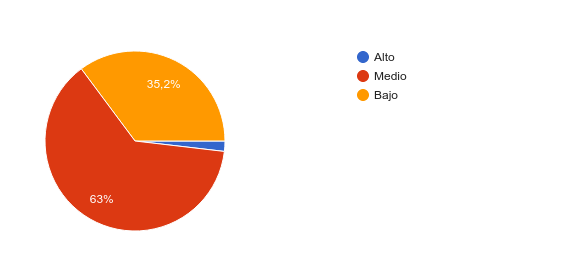
\includegraphics[width=0.8\textwidth]{./Imagenes/Cuestionario/economia.png}
        \caption{Respuesta a pregunta sobre poder adquisitivo}
        \label{fig:economia}
    \end{figure}
    
    \begin{figure}[H]
        \centering 
        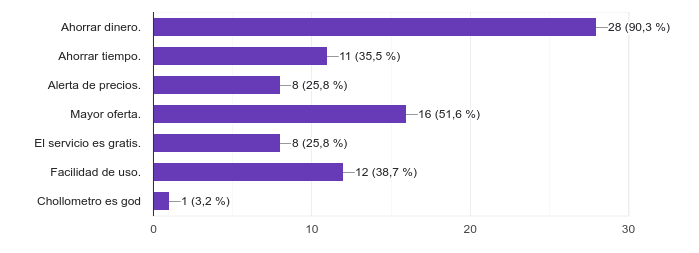
\includegraphics[width=0.7\textwidth]{./Imagenes/Cuestionario/motivo.png}
        \caption{Respuesta a pregunta sobre motivos para viajar}
        \label{fig:motivo}
    \end{figure}
    
    \begin{figure}[H]
        \centering 
        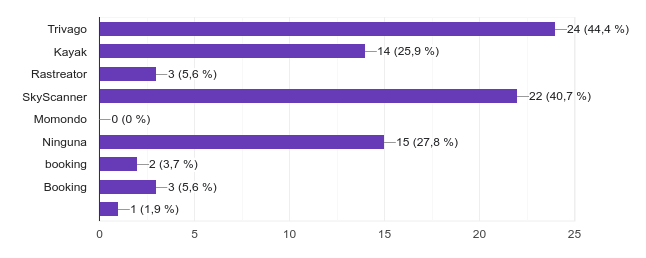
\includegraphics[width=0.7\textwidth]{./Imagenes/Cuestionario/herramientas.png}
        \caption{Respuesta a pregunta sobre qué herramientas usan}
        \label{fig:herramientas}
    \end{figure}

    
    \begin{figure}[H]
        \centering 
        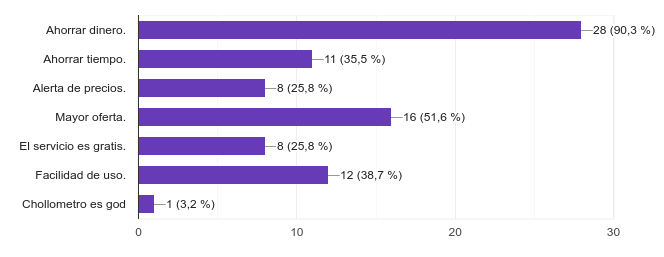
\includegraphics[width=0.7\textwidth]{./Imagenes/Cuestionario/motivos_2.png}
        \caption{Respuesta a pregunta sobre los motivos para usar algún tipo de comparador}
        \label{fig:motivos2}
    \end{figure}


    
    \begin{figure}[H]
        \centering 
        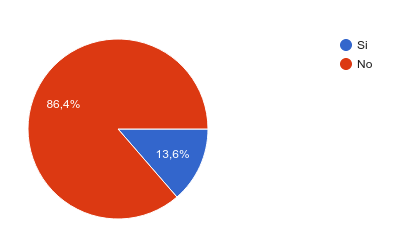
\includegraphics[width=0.65\textwidth]{./Imagenes/Cuestionario/falta_funcionalidad.png}
        \caption{Respuesta a pregunta sobre si echan de menos funcionalidades en los comparadores usados}
        \label{fig:falta_funcionalidades}
    \end{figure}


\subsection{Enlaces}

Dejamos aquí los enlaces al cuestionario en bruto \footnote{Enlace al cuestionario: \url{https://drive.google.com/drive/folders/1btqEATkoGqjZbF4wd30f3foDVuh37EUI?usp=drive_link}} y a los resultados en una hoja de calculo \footnote{ Enlace a los resultados en bruto: \url{https://docs.google.com/spreadsheets/d/1pTHiN6l9IVTqoC7u9HCUusoRIATDoZgKK113m_7aHrQ/edit?usp=drive_link}}

\section{Analisis de la competencia}

Para identificar a la competencia primero debemos conocer cuales son las funcionalidades que va a tener nuestra aplicación para ver cuáles otras del mismo tipo se parecen. Las funcionalidades principales de nuestra aplicación serían:
\begin{itemize}
    \item Búsqueda de alojamiento.
    \item Búsqueda de medio de transporte.
    \item Comparar precios para el mismo viaje.
    \item Comprar billetes y alojamientos.
\end{itemize}

Hemos hecho una búsqueda intensiva de las aplicaciones que pueden tener similitudes con nuestra aplicación.

Vamos a diferenciar entre competencia total y competencia parcial. Las aplicaciones que definimos con competencia total, son aquellas que comparten casi en su totalidad las mismas funcionalidades que nuestra aplicación. Por otro lado, hemos definido como competencia parcial aquellas que comparten alguna funcionalidad similar a nuestra aplicación (solo búsqueda de medios de transporte o solo búsqueda de alojamiento).

\subsection{Competencia total}
\begin{itemize}
    \item\textbf{Kayak.} Es una aplicación que permite comparar alojamientos y medios de transporte, ofrece descripciones detalladas de los destinos con cosas que se pueden hacer en los lugares y cómo moverse por allí. Tiene un mapamundi con etiquetas de los sitios con los precios más baratos. Tiene un 1,8 de valoración sobre 5.
    \item\textbf{eDreams.} Es un comparador de viajes que ofrece búsqueda de transporte y alojamiento y además ofrece el paquete conjunto de las dos y también permite alquiler de coche. Tiene servicio prime para reducir el coste de los viajes.Tiene un 4 de valoración sobre 5.
    \item\textbf{Momondo.} Es un comparador de vuelos, alojamiento y ofrece viajes completos. Tiene una opción de alertas de precios. Tiene un 4 sobre 5 de valoración.
    \item\textbf{SkyScanner.} Es una aplicación para buscar transporte y alojamiento en un destino determinado en unas fechas determinadas ofrece las últimas ofertas y tiene una sección de recomendaciones. Tiene un 3,9 sobre 5 de valoración.
\end{itemize}

\subsection{Competencia parcial:}
\begin{itemize}
    \item\textbf{Trivago.} Es una aplicación para buscar y comparar alojamientos, tiene un sistema de opiniones para valorar el alojamiento, ofrece ofertas, tiene diferentes opciones para encontrar un alojamiento adecuado para las necesidades del usuario. Tiene un 2,8 de valoración sobre 5.
    \item\textbf{Iberia.} Es una aplicación de la aerolínea que permite comparar vuelos de Iberia o de sus filiales. también tiene Iberia plus con un sistema de puntos para obtener descuentos. Tiene un 3 de valoración sobre 5
    \item\textbf{Booking.} Esta web permite comparar y comprar sólo alojamiento, tiene colaboración con aerolíneas como Iberia para hacer descuentos. Tiene un 1,2 de valoración sobre 5.
\end{itemize}

\subsection{Dimensiones}

\textbf{Comparar transporte.} Realizar una comparación de múltiples medios de transporte en unas fechas. [Respuesta binaria, tabla \ref{table:comp-transporte}]
\begin{itemize}
    \item Vuelos
    \item Trenes
    \item Buses
    \item Flexibilidad de fechas 
    \item Filtros de búsqueda 
    \item Alquiler de coche 
\end{itemize}

\begin{table}[H]
    \centering
    \begin{tabular}{l|l|l|l|l|l|l|}
    \cline{2-7}
                                     & Vuelos & Trenes & Buses & Flexibilidad de fechas & Filtros de búsqueda & Alquiler de coche \\ \hline
    \multicolumn{1}{|l|}{Kayak}      & Si     & Si     & Si    & Si                     & Si                  & Si                \\ \hline
    \multicolumn{1}{|l|}{eDreams}    & Si     & Si     & No    & No                     & Si                  & Si                \\ \hline
    \multicolumn{1}{|l|}{Momondo}    & Si     & Si     & Si    & Si                     & Si                  & Si                \\ \hline
    \multicolumn{1}{|l|}{SkyScanner} & Si     & No     & No    & No                     & Si                  & Si                \\ \hline
    \multicolumn{1}{|l|}{Trivago}    & No     & No     & No    & No                     & No                  & No                \\ \hline
    \multicolumn{1}{|l|}{Iberia}     & Si     & No     & No    & Si                     & Si                  & No                \\ \hline
    \multicolumn{1}{|l|}{Booking}    & No     & No     & No    & No                     & No                  & No                \\ \hline
    \end{tabular}
    \caption{Tabla de posibilidad de comparación de transportes entre distintas plataformas}
    \label{table:comp-transporte}
\end{table}

\textbf{Comprar transporte.} Poder comprar un medio de transporte previamente comparado. [Respuesta binaria, tabla \ref{table:comprar-transporte}]

\begin{itemize}
    \item Sistema de puntos
    \item Suscripción prime 
    \item Ecologismo 
    \item Seguros
\end{itemize}

\begin{table}[H]
    \centering
    \begin{tabular}{l|l|l|l|l|}
    \cline{2-5}
                                     & Sistemas de puntos & Suscripción prime & Ecologismo & Seguros \\ \hline
    \multicolumn{1}{|l|}{Kayak}      & No                 & No                & No         & Si      \\ \hline
    \multicolumn{1}{|l|}{eDreams}    & Si                 & Si                & Si         & Si      \\ \hline
    \multicolumn{1}{|l|}{Momondo}    & No                 & No                & No         & Si      \\ \hline
    \multicolumn{1}{|l|}{SkyScanner} & Si                 & Si                & Si         & Si      \\ \hline
    \multicolumn{1}{|l|}{Trivago}    & No                 & No                & No         & No      \\ \hline
    \multicolumn{1}{|l|}{Iberia}     & Si                 & Si                & No         & Si      \\ \hline
    \multicolumn{1}{|l|}{Booking}    & No                 & No                & No         & No      \\ \hline
    \end{tabular}
    \caption{Tabla comparativa sobre distintas características de los sistemas de compra}
    \label{table:comprar-transporte}
    \end{table}

\textbf{Comparar alojamiento.} Realizar una comparación dde múltiples alojamientos en unas fechas. [Respuesta binaria, tabla \ref{table:comp-aloj}]

\begin{itemize}
    \item Opiniones 
    \item Valoración con estrellas 
    \item Filtros de búsqueda 
    \item Flexibilidad de fechas
\end{itemize}

\begin{table}[H]
    \centering
    \begin{tabular}{l|l|l|l|l|}
    \cline{2-5}
                                     & Opiniones & Valoración con estrellas & Filtros de búsqueda & Flexibilidad de fechas \\ \hline
    \multicolumn{1}{|l|}{Kayak}      & Si        & Si                       & Si                  & Si                     \\ \hline
    \multicolumn{1}{|l|}{eDreams}    & Si        & Si                       & Si                  & No                     \\ \hline
    \multicolumn{1}{|l|}{Momondo}    & Si        & Si                       & Si                  & Si                     \\ \hline
    \multicolumn{1}{|l|}{SkyScanner} & Si        & Si                       & Si                  & No                     \\ \hline
    \multicolumn{1}{|l|}{Trivago}    & Si        & Si                       & Si                  & No                     \\ \hline
    \multicolumn{1}{|l|}{Iberia}     & No        & No                       & No                  & No                     \\ \hline
    \multicolumn{1}{|l|}{Booking}    & Si        & Si                       & Si                  & Si                     \\ \hline
    \end{tabular}
    \caption{Tabla de funcionalidades de la comparación de viajes}
    \label{table:comp-aloj}
    \end{table}

\textbf{Comprar alojamiento.} Poder comprar un alojamiento previamente comparado. [Respuesta vinaria, tabla \ref{table:comprar-aloj}]

\begin{itemize}
    \item Sistema de puntos 
    \item Suscripción prime 
    \item Seguros
\end{itemize}

\begin{table}[H]
    \centering
    \begin{tabular}{l|l|l|l|}
    \cline{2-4}
                                     & Sistemas de puntos & Suscripción prime & Seguros \\ \hline
    \multicolumn{1}{|l|}{Kayak}      & No                 & No                & Si      \\ \hline
    \multicolumn{1}{|l|}{eDreams}    & No                 & Si                & Si      \\ \hline
    \multicolumn{1}{|l|}{Momondo}    & No                 & No                & Si      \\ \hline
    \multicolumn{1}{|l|}{SkyScanner} & Si                 & Si                & Si      \\ \hline
    \multicolumn{1}{|l|}{Trivago}    & No                 & No                & No      \\ \hline
    \multicolumn{1}{|l|}{Iberia}     & No                 & No                & No      \\ \hline
    \multicolumn{1}{|l|}{Booking}    & No                 & No                & No      \\ \hline
    \end{tabular}
    \caption{Tabla de comparación de las distintas funcionalidades de la compra / reserva de alojamientos}
    \label{table:comprar-aloj}
    \end{table}

\subsection{Recomendaciones de acción}

A raíz de los resultados obtenidos en las tablas vamos a sacar unas recomendaciones de acción que nos permitan saber qué nos quiere decir este estudio.

\begin{itemize}
    \item Todas las páginas que ofrecen servicio de comparar transporte tienen buenos filtros de búsqueda, debemos incluir un buen sistema de filtros.Todas ofrecen como mínimo poder buscar vuelos, algunas incluyen trenes y buses en las búsquedas, sería interesante incluir todas en nuestra aplicación. No todas ofrecen poder buscar con flexibilidad de fechas, así que vemos interesante incluir flexibilidad de fechas en nuestra aplicación. No todas ofrecen servicio de alquiler de coche, es interesante incluirlo en la aplicación.
    \item Muy pocas páginas de las estudiadas ofrecen un sistema de puntos y suscripción prime, puede ser interesante incluirlo en nuestra aplicación. Solo dos de las páginas estudiadas ofrecen opciones de ecologismo, valoramos que no es tan interesante incluirlo en nuestra aplicación. Casi todas ofrecen un sistema de seguros a la hora de comprar un medio de transporte, es interesante incluirlo.
    \item Todas las aplicaciones utilizan un sistema de opiniones y de valoración gráfica con estrellas a la hora de mostrar los alojamientos comparados. Es muy interesante incluir esto en nuestra aplicación. Así como filtros de búsqueda también tienen todas, es interesante incluir buenos filtros. No todas ofrecen flexibilidad de fechas a la hora de comparar los alojamientos, es interesante incluirlo en nuestra aplicación.
    \item Para comprar alojamientos solo una aplicación incluye un sistema de puntos para comparar alojamientos, puede no ser interesante incluir un sistema de puntos para los alojamientos. De las páginas estudiadas para comprar alojamiento, dos de ellas utilizan sistema de prime, es interesante incluirlo. De estas páginas para comprar alojamiento todas tienen un sistema de seguros, es muy interesante incluirlo.
\end{itemize}

\section{Mapas de empatía}

Los mapas de empatía son una técnica de investigación que permite conocer más en profundidad al usuario con el que se está tratando. Es una de las técnicas que se está comenzando a implementar actualmente en la mayoría de empresas y consta de una plantilla dividida por sectores en los que cada uno de ellos representa distintos “estímulos” que percibe el usuario. \\

En nuestro caso, hemos utilizado una de las plantillas proporcionadas por Creately, que sugiere que dividamos el espacio en 7 regiones. Cada una de estas regiones, como vamos a ver, se va a centrar en un aspecto distinto de la personalidad del usuario. Concretamente hemos elegido esta porque dentro de la oferta de plantillas de la aplicación era la más comprensible y completa, ya que se centraba en varios aspectos de la personalidad, como lo que hacen los usuarios o lo que sienten, motivo por el que optamos por trabajar a partir de ella. \\

Dentro de esta plantilla, como se ha visto, existen 7 regiones claramente diferenciadas y en la que se responde a una pregunta. Estas secciones son las siguientes:
\begin{enumerate}
    \item {\textbf{Who are we empathizing with? (?`Con quién estamos empatizando?)}}.  Describe brevemente al usuario y el papel que desempeña dentro de nuestra aplicación.
    \item {\textbf{What do they need to do? (?`Qué necesitan hacer?)}}. Explica los procesos que sigue el usuario para conseguir su objetivo y las herramientas que necesita para ello. A su vez también expone las razones por las que se considera que el usuario ha logrado su objetivo.
    \item {\textbf{What do they see? (?`Qué ven?)}}. Es una de las fases en las que hay que ponernos en la piel del usuario y en base a lo contado en las entrevistas / cuestionarios, intentar describir cómo ve los procesos y a las personas, identificando las dificultades que observa.
    \item {\textbf{What do they say? (?`Qué dicen?)}}. En este apartado vamos a extraer algunas de las principales frases que han sido obtenidas durante la fase de entrevistas y que nos van a poner en contexto de la situación del entrevistado.
    \item {\textbf{What do they do? (?`Qué hacen?)}}. Se trata de las acciones que realiza el usuario, deducidas en base a la información obtenida en las entrevistas.
    \item {\textbf{What do they hear? (?`Qué escuchan?)}}. En esta sección vamos a volver a ponernos en la piel del usuario para poder conocer aquellos estímulos auditivos que puede recibir (de familia y amigos por ejemplo).
    \item {\textbf{What do they think and feel? (?`Qué sienten o escuchan?)}}. Por último, vamos a centrarnos en los pensamientos y sentimientos del usuario, clasificándolos en función de lo perjudiciales o beneficiosos que van a resultar y aportando un pensamiento o sugerencia que hayan tenido de mejora en la entrevista.
\end{enumerate}

 Una vez seleccionada y descrita la plantilla definitiva con la que vamos a trabajar, comenzamos a completar los distintos mapas de los entrevistados. Dentro de cada una de ellas hemos ido añadiendo tarjetas con pequeñas piezas de información referente a la pregunta del correspondiente sector, completando poco a poco con pequeñas piezas de información. \\

Muchas de estas preguntas han sido respondidas con las respuestas proporcionadas por los usuarios en sus entrevistas, pero existen otras (como la número 3), en la que tendremos que servirnos de los datos obtenidos en las entrevistas o en los cuestionarios, poniéndonos en la piel del usuario intentando dar respuesta a estas cuestiones.
\subsection{Resultados}
\begin{figure}[H]
    \centering 
    \includegraphics[width=0.9\textwidth]{./mapas_empatia/Mapa de Empatía - Madi.pdf}
    \caption{Mapa de empatía de la entrevista 1}
    \label{fig:mapa_madi}
\end{figure}

\begin{figure}[H]
    \centering 
    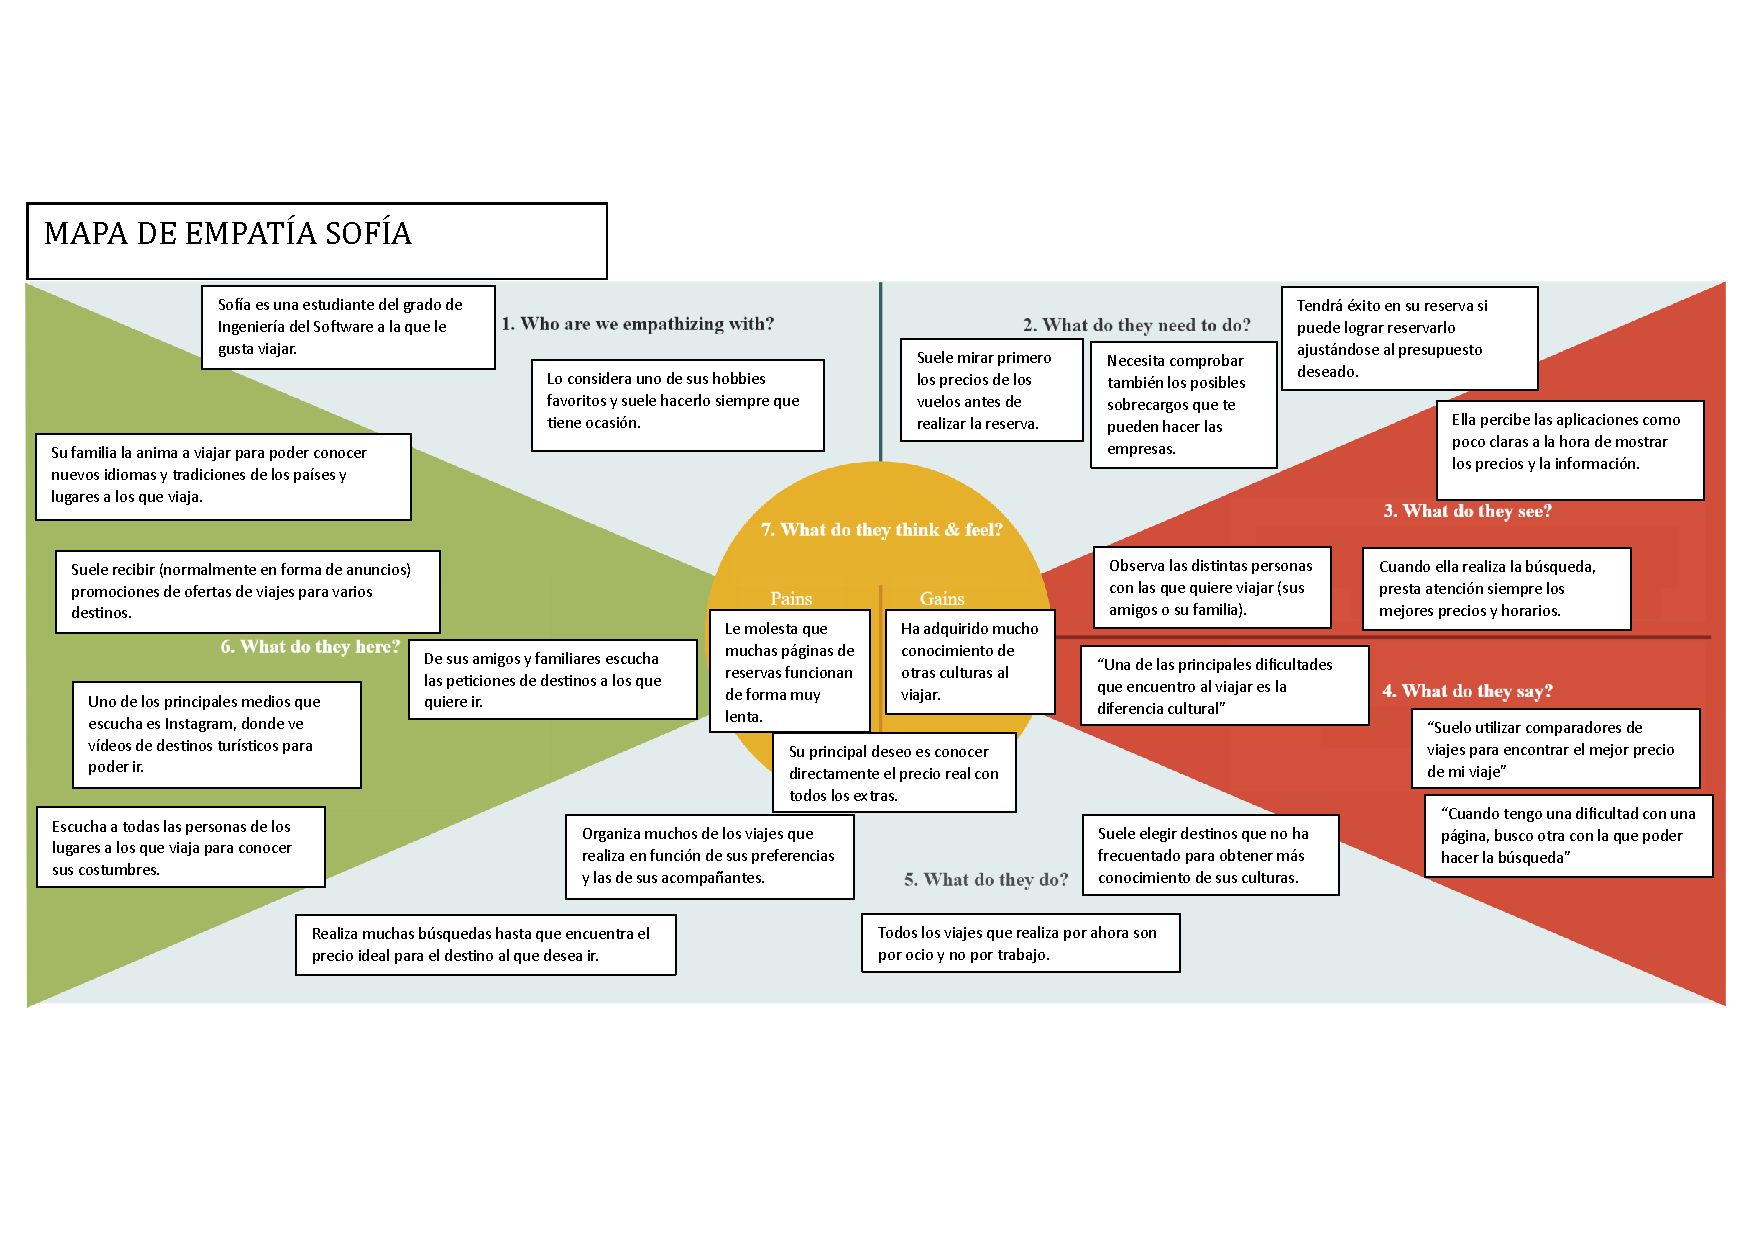
\includegraphics[width=0.9\textwidth]{./mapas_empatia/Mapa de Empatía - Sofía.pdf}
    \caption{Mapa de empatía de la entrevista 2}
    \label{fig:mapa_sofia}
\end{figure}

\begin{figure}[H]
    \centering 
    \includegraphics[width=0.9\textwidth]{./mapas_empatia/Mapa de Empatía - Alberto.pdf}
    \caption{Mapa de empatía de la entrevista 3}
    \label{fig:mapa_alberto}
\end{figure}

\begin{figure}[H]
    \centering 
    \includegraphics[width=0.9\textwidth]{./mapas_empatia/Mapa de Empatía - Beatriz.pdf}
    \caption{Mapa de empatía de la entrevista 4}
    \label{fig:mapa_bea}
\end{figure}

\section{Listado de factoides}

Tras realizar toda la investigación anterior, presentamos los factoides que hemos sacado de cada parte:

\textbf{Factoides de Madi:}

\begin{itemize}
    \item Madi es secretaria de la FEDDI y lleva 16 años trabajando allí.
    \item Madi se encarga de organizar los viajes cuadrando horarios y comprando billetes.
    \item Madi compra billetes a través de Renfe, Air Europa o Iberia porque le sale más económico que en un comparador.
    \item Madi se encarga de los viajes de campeonatos internacionales que les recepciona, les recoge y les lleva al punto de encuentro. Los nacionales los llevan los clubes.
    \item Madi ve que el problema principal para los deportistas es la dependencia de sus padres y entrenadores, el manejo de las aplicaciones y el internet y para algunos necesitan acompañante.
    \item Madi considera que necesitan acompañantes porque tienen problemas para orientarse y no se manejan bien.
    \item Para Madi las dificultades dependen mucho del grado de discapacidad.
    \item Madi no usa aplicaciones, sólo compra en páginas oficiales de la aerolínea.
    \item Madi utiliza la agencia de viajes Betravel para vuelos internacionales.
    \item Madi descarta Ryanair.
    \item Madi no utiliza comparadores porque ya tiene localizadas dos compañías y Renfe que ofrecen el servicio de acompañamiento de Aena.
    \item Madi tiene en cuenta el precio y la variedad de horarios para coger un billete.
    \item Madi no se fija en más facilidades, esos son los atletas.
    \item Madi considera que el comparador debe ser muy simple (lugar, destino y fecha).
    \item A Madi le parece importante que se pueda ver qué tipos de servicios de acompañantes ofrecen.
\end{itemize}


\textbf{Factoides de Sofia:}

\begin{itemize}
    \item Sofía tiene 21 años.
    \item A Sofía le gusta viajar y desde pequeña ha querido conocer las diferentes partes del mundo.
    \item Sofía viaja a menudo, tanto fuera como dentro de España.
    \item A Sofía le encantaría poder viajar más.
    \item Sofía usa tanto automóviles como coches, trenes y autobuses en sus viajes dependiendo del sitio al que viaje.
    \item Sofía prefiere usar autobuses solo cuando viaje distancias cortas o medias.
    \item Sofía ha hecho viajes de varios tipos. Desde intercambios lingüísticos a viajes familiares o con amigos, para conocer nuevas ciudades o relajarse.
    \item A Sofía le gusta ir alternando entre viajar sola, con familia o con amigos, disfruta de todas.
    \item Sofía no recuerda haber tenido ningún problema viajando, aunque admite que cuando viaja lo hace con la mente más abierta de lo que la tiene normalmente.
    \item Sofía a veces organiza los viajes que hace y a veces no.
    \item Sofía busca viajes económicamente accesibles.
    \item Sofía utiliza varios comparadores de viajes a la hora de organizar un viaje. Por ejemplo: Kayak, Skyscanner, Trivago.
    \item A Sofía le gustaría que los comparadores de viajes mostraran el precio final del billete, con los posibles extras incluidos, piensa que es un punto a mejorar.
    \item Sofía prefiere usar aplicaciones web a aplicaciones móviles, y suele hacer estas gestiones desde el ordenador.
    \item Sofía piensa que algunos comparadores son tediosos a la hora de usar, ya que algunos tardan mucho en cargar o te redirigen a otras páginas.
    \item Cuando le ha ocurrido esto, Sofía ha optado por usar otro comparador que no tuviera estos problemas.
    \item Como aportación, a Sofía le gustaría que los comparadores incluyeran el precio final de los billetes, desglosados con los diferentes conceptos.
    \item Sofía considera que los comparadores de viajes son bastante accesibles, pero que quizás aclarar algunas cosas en las webs o los anuncios de spam en las webs pueden molestar a personas con discapacidad intelectual.
    \item Sofía considera que Whatsapp es una aplicación accesible.
\end{itemize}


\textbf{Factoides de Alberto:}

\begin{itemize}
    \item Alberto tiene 22 años y es informático.
    \item Alberto no tiene discapacidad.
    \item Alberto se desenvuelve bien con las tecnologías y le parecen fáciles de usar.
    \item A Alberto le gusta viajar para descubrir historias, paisajes y nuevas culturas.
    \item Alberto viaja exclusivamente por ocio.
    \item Alberto viaja una vez al mes.
    \item A Alberto le gustaría viajar más, más adelante fuera de España.
    \item Alberto usa normalmente vehículo propio para viajar.
    \item Alberto hace 7 años que no viaja en avión.
    \item Alberto usa ocasionalmente taxis, pero prefiere el transporte público.
    \item Alberto descarta el uso de Uber.
    \item Alberto suele viajar con su pareja.
    \item Alberto prepara o busca un itinerario antes de viajar, incluso toma apuntes de paradas por si le falla el móvil o gps, le parece tedioso igualmente y se encarga con su pareja.
    \item Alberto sólo usa comparadores para alojamientos mirando lo visual que sea, la localización y el precio.
    \item Alberto usa Booking y le parece incómodo que le obliguen a poner fechas para ver el precio, prefiere ver el precio directamente.
    \item A Alberto le gusta ver pocas ofertas y más relevantes, y no ver muchas ofertas.
\end{itemize}


\textbf{Factoides de Beatriz:}
\begin{itemize}
    \item Beatriz tiene 21 años.
    \item Beatriz se desenvuelve bien con las tecnologías y declara usarlas a diario.
    \item A Beatriz le gusta viajar para conocer otros lugares y culturas.
    \item Beatriz viaja una vez al año, sobre todo dentro de España, y fuera de España una vez cada dos años.
    \item A Beatriz le gustaría viajar más; son razones económicas y de tiempo lo que se lo impide.
    \item Suele viajar en coche o en avión para distancias más largas.
    \item Beatriz suele viajar para visitar a familiares o por razones de ocio.
    \item Beatriz suele viajar acompañada.
    \item Cuando no viaja con su familia, Beatriz suele organizar los viajes que hace.
    \item Beatriz se fija sobretodo en el precio a la hora de tomar una decisión, por ejemplo, para comprar un vuelo.
    \item En su último viaje, Beatriz optó por usar una aplicación (eDreams) debido a que tenían un programa con prueba gratuita con el que sus vuelos le salieron más baratos.
    \item Beatriz prefiere los vuelos de ida tempranos y los de vuelta más tarde.
    \item A la hora de hacer la reserva, Beatriz cree que lo más tedioso son todas las pantallas que tienes que atravesar en las que te ofrecen todo tipo de servicios extra, alguno incluso ofreciéndose dos veces.
    \item A Beatriz también le gustaría que los comparadores pusieran un mensaje más claro en el caso de que ida y vuelta sean desde aeropuertos distintos.
    \item Las aplicaciones que más usa Beatriz son Chrome, Whatsapp y Discord.
    \item Google es su navegador favorito, principalmente porque lo lleva usando mucho tiempo y está acostumbrada, pero también debido a la conectividad con otros servicios en su móvil y porque considera que es lo mejor en cuanto a desarrollo web; también le gusta su estética.
    \item El comparador favorito de vuelos de Beatriz es el comparador de Google.
    \item Beatriz considera que los comparadores de vuelos pueden no ser accesibles para personas que no tengan mucha soltura con las tecnologías.
    \item Beatriz considera que eDreams es muy estético, más que el comparador de Google o que otros.
    \item Como aportación, a Beatriz le gustaría que los comparadores te sugirieran vuelos desde sitios cercanos a los que estás buscando, sobretodo si están son más económicos.
\end{itemize}


\textbf{Factoides del cuestionario:}

\begin{itemize}
    \item La mitad de los usuarios tienen entre 19 y 25 años y la otra mitad entre 26 y 65 años.
    \item La mayoría de los encuestados viven en la ciudad, pocos en pueblos.
    \item Dos tercios de los encuestados tienen un poder adquisitivo medio. Un tercio, bajo y muy pocos, alto.
    \item La mayoría de los encuestados les gusta viajar, pocos no.
    \item La mayoría de los encuestados le gusta viajar por conocer nuevos lugares y los pocos que no, es por la gente o por no parar de moverse.
    \item La mayoría de los encuestados viajan al menos una vez al año, el resto viajan al menos una vez al mes y muy poco no viajan.
    \item La mayoría de los encuestados le gustaría viajar más, el resto no.
    \item Todos los encuestados disfrutan cuando viajan.
    \item Los medios de transporte que usan los encuestados son coche propio, transporte público y aéreo.
    \item Los encuestados suelen viajar por ocio, pocos por trabajo.
    \item Las herramientas que más utilizan los encuestados son Trivago, Kayak y SkyScanner. Hay un tercio de los encuestados que no usan ninguna.
    \item Los comparadores de viajes (Trivago, Kayak, Rastreator, SkyScanner, Momondo) son de fácil uso.
    \item Un quinto de los encuestados tienen alguna discapacidad reconocida.
    \item Los encuestados con discapacidad la mayoría tienen discapacidad física y el resto es intelectual o mental.
    \item Los encuestados con discapacidad dos tercios necesitan adaptaciones para sus viajes como para sillas de ruedas.
    \item La mayoría de los encuestados con discapacidad a veces planifican y el resto o nunca o siempre.
    \item Un tercio de los encuestados con discapacidad encuentran dificultad en el proceso de búsqueda por la accesibilidad.
    \item La mayoría de los encuestados con discapacidad no les supone una dificultad buscar medio de transporte, hacer, comparar y ver las ventajas/desventajas de las rutas o comparar precios.
    \item La mitad de los encuestados con discapacidad no usan comparadores de viajes o similares.
    \item Los encuestados con discapacidad que han usado comparadores la mayoría ha desistido.
    \item Para los encuestados con discapacidad les parece complejo solicitar ayuda dentro de la aplicación de viajes.
    \item La inmensa mayoría de los encuestados sin discapacidad ha viajado en el último año.
    \item La mayoría de los encuestados sin discapacidad hace búsqueda de viaje.
    \item Dos tercio de los encuestados sin discapacidad han utilizado un comparador de viajes.
    \item El motivo principal de los encuestados sin discapacidad es ahorrar dinero. También está mayor oferta, facilidad de uso y ahorra tiempo.
    \item Los encuestados sin discapacidad no tienen problemas con los comparadores.
    \item A los encuestados sin discapacidad les supone una dificultad en el tema de la accesibilidad tener que hacer muchas operaciones para llegar a un objetivo.
    \item Los encuestados están de acuerdo en su mayoría de que está bien la accesibilidad salvo por la ausencia de ayudas al rellenar.
    \item La mayoría de los encuestados no ha echado en falta ninguna funcionalidad.
\end{itemize}


\textbf{Factoides del análisis de competencia}

\begin{itemize}
    \item Las funcionalidades buscadas en otras aplicaciones son búsqueda de alojamiento, búsqueda de medio de transporte, comparar precios para el mismo viaje y comprar billetes y alojamientos.
    \item La competencia total a la aplicación está formada principalmente por kayak, eDreams, Momondo y SkyScanner.
    \item La competencia parcial a la aplicación está formada por Trivago, Iberia y Booking.
    \item La mayor diferencia entre Trivago/Booking y nuestra aplicación es que Trivago y Booking son aplicaciones exclusivamente de alojamiento.
    \item La mayor diferencia entre Iberia y nuestra aplicación es que Iberia solo ofrece búsqueda de vuelos de Iberia y no permite buscar alojamiento u otros tipos de transporte.
    \item La aplicación eDreams no permite buscar buses ni tiene flexibilidad de fechas.
    \item SkyScanner solo ofrece como modelo de transporte vuelos y no tiene flexibilidad de fechas.
    \item Kayak y Momondo no tienen sistema de puntos ni suscripción prime.
    \item Todas las páginas para comparar transporte tienen un buen sistema de filtración de opciones.
    \item Todas las aplicaciones ofrecen como mínimo poder buscar vuelos, algunas incluyen trenes y buses en las búsquedas.
    \item No todas las aplicaciones permiten buscar con flexibilidad de fechas.
    \item Todas las aplicaciones tienen un sistema de opiniones y de valoración con estrellas.
\end{itemize}
